\documentclass[10pt]{article}
\usepackage{graphicx}
\usepackage[T1]{fontenc}
\usepackage[utf8]{inputenc}
\usepackage[letterpaper,margin=1in]{geometry}
\usepackage[parfill]{parskip}
\usepackage[europeanresistors, american voltage]{circuitikz}

\begin{document}

\title{\textbf{\Large{\textsc{ECE320:} Fields and Waves}} \\ \Large{Lab 1 Report: Waves on Transmission Lines}}
\author{Alp Tarım, Pranshu Malik}


\maketitle

\section{Introduction}
This assignment was about exploring the characteristics of transmission lines (abbrv. T.L.), studying voltage and current 
propagation along the T.L.s, as well as depedance on loads. Introduction to the lab and its purpose. The following is the reflection coefficient for a transmission line

% \[
%     \label{reflection_coefficient}
%     \Gamma = \frac{Z_L - Z_0}{Z_L + Z_0}
% \]

\section{Determining the Characteristic Impedance, $Z_0$}

We varied the load on the switch box until we saw little or no traces of reflected waves.
This was at $Z_L = 50 \Omega$ which is also equal to the charactertic impedance 
since we know that the reflections nullify when $Z_L = Z_0$. The corresponding waveforms
captured at the generator input (channel 1, yellow) and the transmission line input (channel 2, green) 
are shown in Figure 1.

\begin{figure}[h]
    \centering
    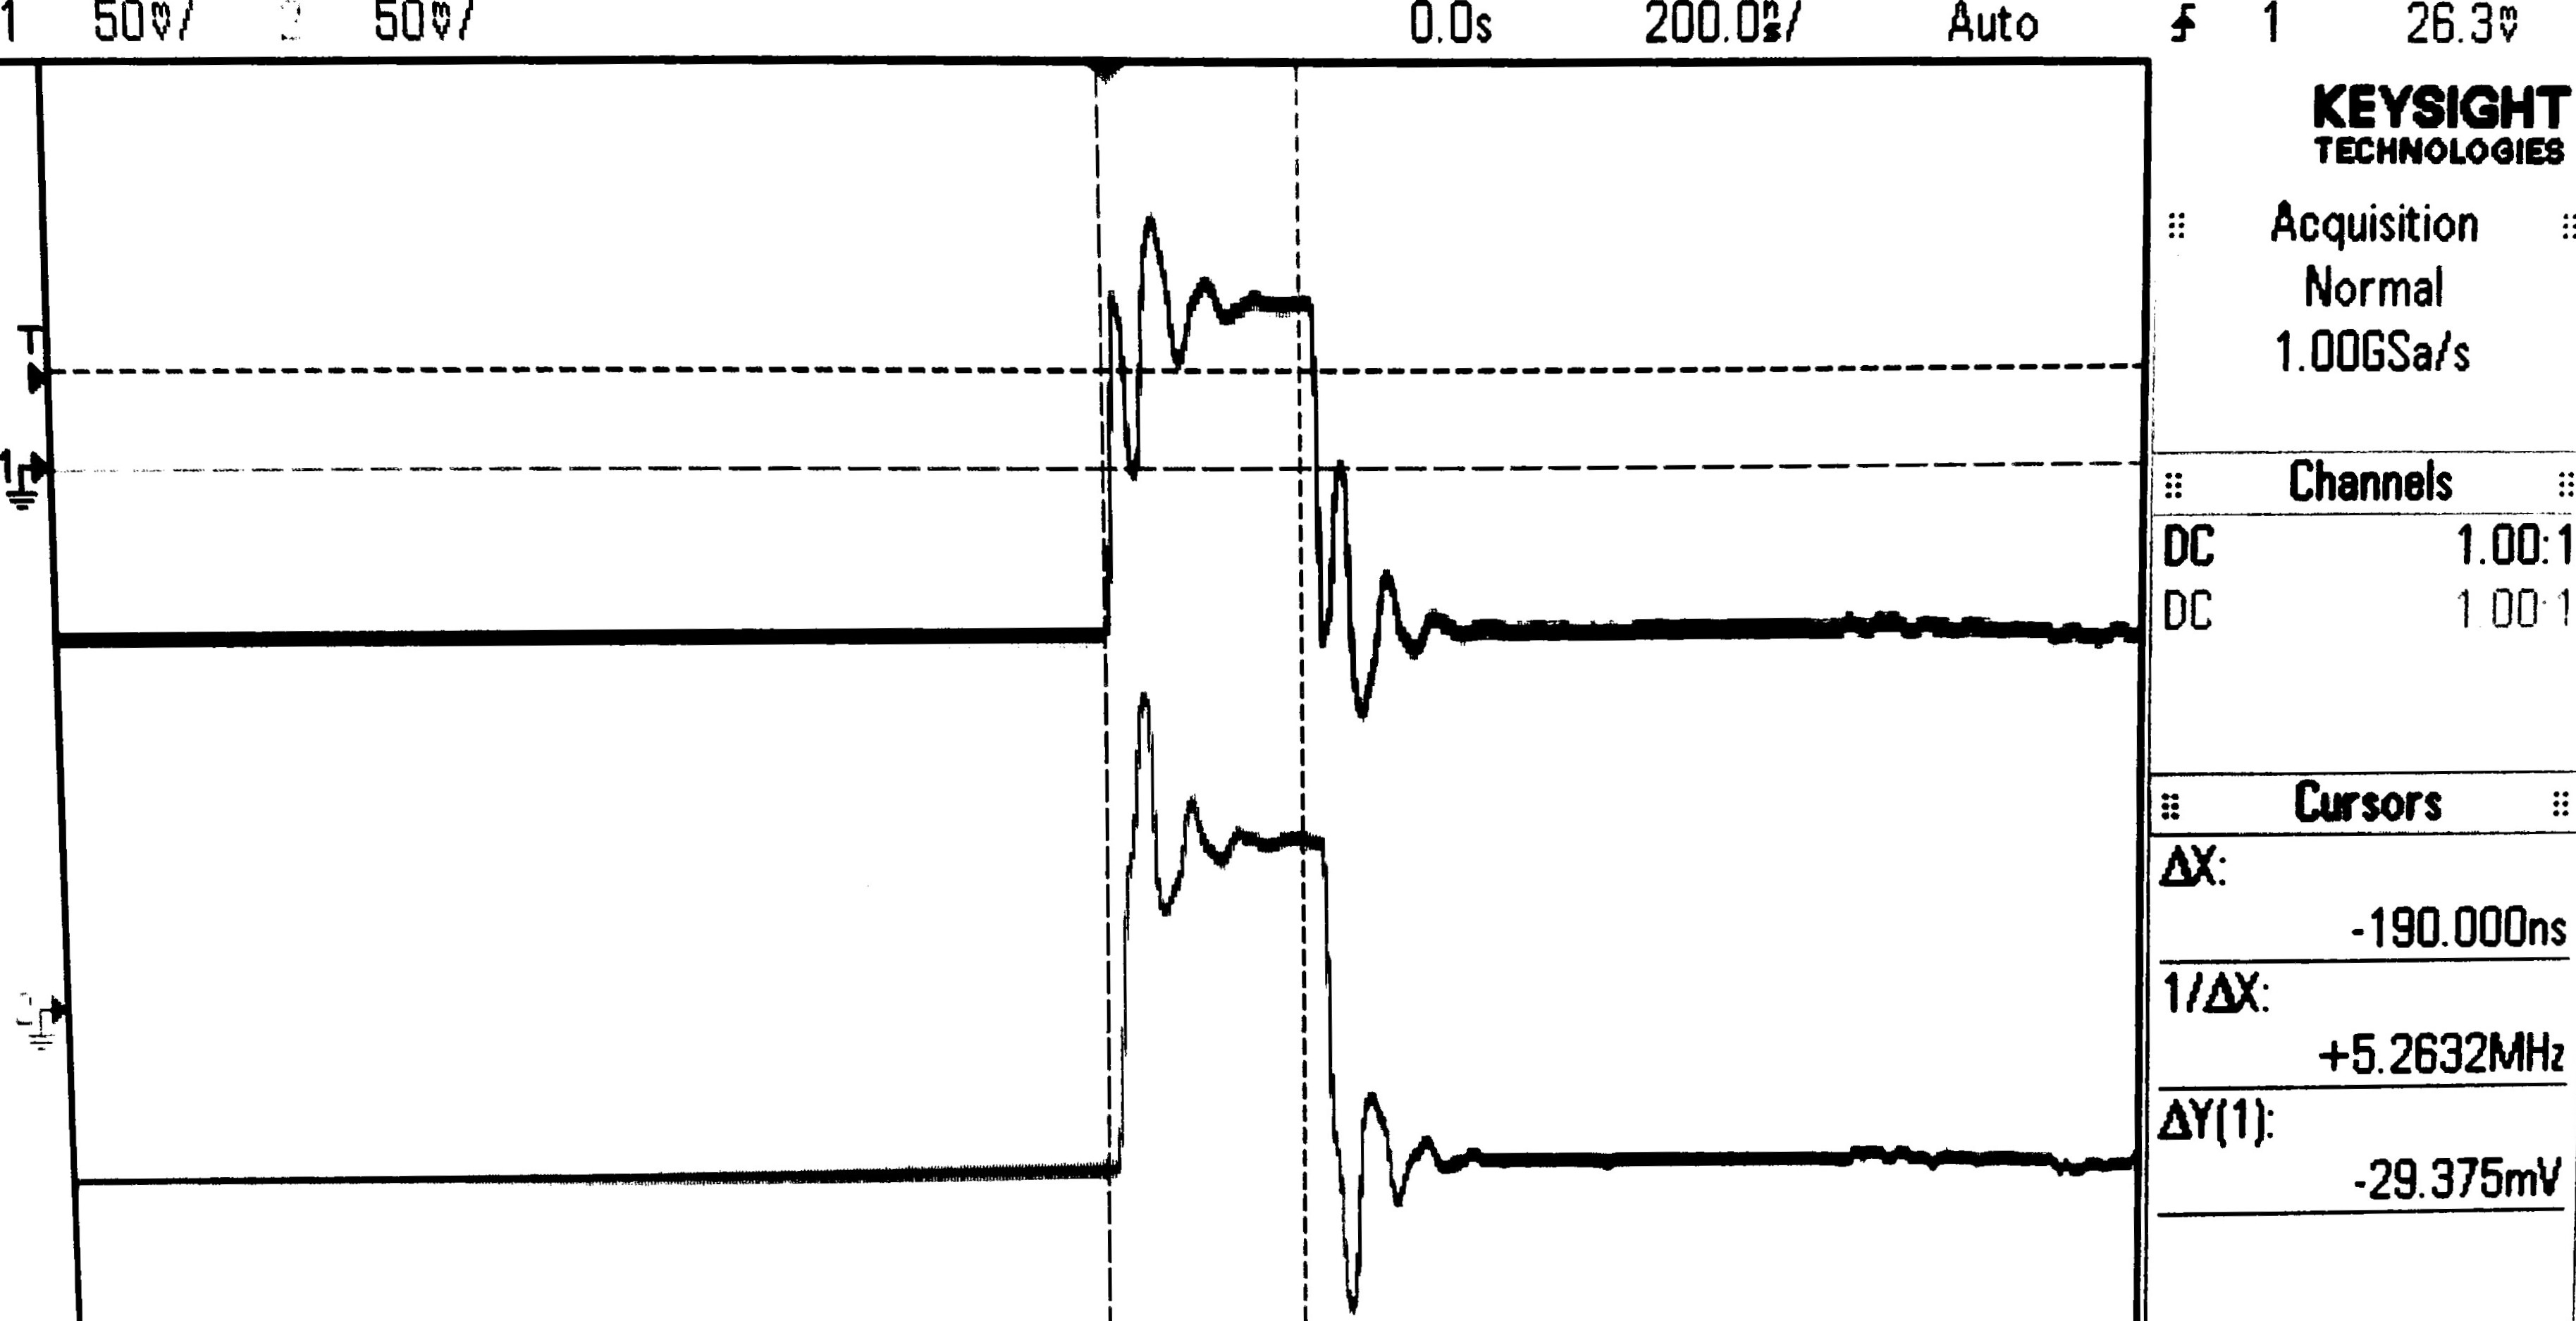
\includegraphics[width=6.0cm]{../photos/lab1/load_matched.jpg}
    \caption{Transmission line terminated with load equal to $Z_0$}
    \label{simulation_figure}
\end{figure}

\section{Determining $Z_0$ using $\frac{\tilde V^+(z=0)}{\tilde I^+(z=0)}$}

As seen in the picture the voltage at $v_g$ is 154mV and $v_1$ is equal to 51mV. Assuming the resistance in between is $100\Omega$ 
 $i_l$ = $\frac{0.154-0.051}{100}$ = $1.03*10^-3$A. Which means $Z_0=\frac{v_1}{i_l}=\frac{0.051}{1.03*10^-3}=49.51\Omega~50\Omega $

\begin{figure}[h] \centering
    \begin{circuitikz} \draw
        (0,2) to [sqV, l_=$\tilde V_g$] (0, 0) -- (2,0)
        to [tline, l_=Transmission Line, *-o] (7,0)
        to [R, l_=$Z_L$] (7, 2)
        to [tline, l_=${Z_0, \beta}$, o-*] (2.8,2)
        to [short, i_=${\tilde I(z=0) v(z=0)}$] (2,2)
        to [R, l_=$Z_g$] (0, 2);

        \draw (2,2) to[sV, l=\footnotesize{CH1}, color=gray] (2,0);
    \end{circuitikz}
    \caption{Pulse }
    \label{circuit_diag}    
\end{figure}

Thus, we can see something there.

\section{Observation of Travelling Waves}

We know that the phase velocity of an electromagentic wave in space with magnetic permeability, $\mu$,
and electric permittivitty, $\epsilon$  is given by: 

$$v_p = \frac{1}{\sqrt{\mu \epsilon}}$$


\section{Conclusion}

Lorem ipsum dolor sit amet, consectetur adipisicing elit, sed do eiusmod tempor
incididunt ut labore et dolore magna aliqua. Ut enim ad minim veniam, quis
nostrud exercitation ullamco laboris nisi ut aliquip ex ea commodo consequat.
Duis aute irure dolor in reprehenderit in voluptate velit esse cillum dolore eu
fugiat nulla pariatur.

\section{Notes}

All pictures taken during the lab were post-processed in a batch using a custom script
that bit-wise inverted the pixels and the thresholded to produce a binarized image. No
adjustments or modifications were made to the readings, for which the oscilloscope's measurements
are also shown alongside the waveforms.

\end{document}